\documentclass[10pt]{report}

\usepackage{stan-talks}

\begin{document}
\sf%
\vspace*{-12pt}
%
\noindent
\spc{\Huge\bfseries \color{MidnightBlue}{WALNUTS:}}
\\[12pt]
\spc{\LARGE\bfseries \color{MidnightBlue}{Per-leapfrog step size
    adaptation for HMC}}
\\[16pt]
\noindent
\spc{\Large\bfseries \color{MidnightBlue}{Bob Carpenter}}
\\[8pt]
\spc{\large Center for Computational Mathematics}
\\[4pt]
\spc{\large Flatiron Institute}
\\[12pt]
\vfill
\hfill

\includegraphics[height=0.35in]{img/fi-logo.png}
\qquad

\includegraphics[height=0.5in]{img/stan-logo.png}

\sld{Bayesian statistics with Monte Carlo}
\begin{itemize}
\item Bayesian \myemph{posterior inference} given data $y$ with parameters $\theta$:
\begin{eqnarray*}
  \widehat{\theta} & = & \mathbb{E}[\Theta \mid y]
  \\
  \Pr[E \mid y] & = & \mathbb{E}[\textrm{I}_E(\Theta) \mid y]
  \\
  p(\widetilde{y} \mid y) & = & \mathbb{E}[p(\widetilde{y} \mid
                                \Theta) \mid y]
\end{eqnarray*}
\item Expectations involve \myemph{high-dimensional integrals}.
  $$ \mathbb{E}[f(\Theta) \mid y] = \int_\Theta f(\theta) p(\theta
  \mid y) \textrm{d}\theta. $$
\item (Markov chain) \myemph{Monte Carlo solves integrals} with $\theta^{(m)} \sim p(\theta \mid y).$
  $$ \mathbb{E}[f(\Theta) \mid y] \approx \frac{1}{M} \sum_{m=1}^M
  f(\theta^{(m)}) $$
\end{itemize}

\sld{Why NUTS?}
%
\begin{itemize}
\item Hamiltonian Monte Carlo (HMC, 1985), a Markov chain Monte
  Carlo (MCMC) method that \myemph{scales well in dimension}.
  \begin{subitemize}
  \item \myemph{integrated autocorrelation time}$^*$: $\mathcal{O}\left(D^{1/4}\right)$ \qquad \myemph{memory}: $\mathcal{O}(D)$
    \\ \qquad $^*$: times ``constant'' based on condition number (Langmore et al.\ 2020)
 \item Hamiltonian \myemph{gradient flow} overcomes diffusive random walk behavior.
  \end{subitemize}
\item Why wasn't HMC in wide use until the \myemph{no-U-turn sampler}
  (NUTS, 2012)?
  \vspace*{-8pt}
  \begin{subitemize}
  \item NUTS in Stan, PyMC, NumPyro, Turing.jl, Blackjax, NIMBLE, ADMB, etc.
  \end{subitemize}
  \vfill
\item \myemph{Double whammy}:
  \begin{subitemize}
  \item HMC is hard to tune; NUTS brought \myemph{self tuning} and \myemph{general software}.
  \item gradients are hard for applications; \myemph{automatic differentiation} makes it easy.
  \end{subitemize}
\end{itemize}

\sld{What is HMC and why is it hard to tune?}
\begin{itemize}
\item Fictitious physical system with \myemph{position} $\theta \in
  \mathbb{R}^D$ and \myemph{momentum} $\rho \in \mathbb{R}^D$:
  \begin{subitemize}
  \item \myemph{Potential} energy: $U(\theta) = - \log p(\theta)$ for
    \myemph{target density} $p(\theta)$
  \item \myemph{Kinetic} energy: $K(\rho) - \log \textrm{normal}(\rho \mid 0, M)$
  \item \myemph{Hamiltonian} (total energy): $H(\theta, \rho) =
    U(\theta) + K(\rho)$, \quad $p(\theta, \rho) = \exp\left( -H(\theta, \rho)\right)$
  \end{subitemize}
\item \myemph{HMC iteration} from position $\theta(0)$:
  \begin{subitemize}
  \item \myemph{Sample momentum}: $\rho(0) \sim \textrm{normal}(0, M)$
  \item \myemph{Evolve Hamiltonian exactly}: $(\theta(0), \rho(0))$ 
    to $(\theta(t), \rho(t))$, return $\theta(t)$.
  \end{subitemize}
\item In practice, can't solve exactly, so discretize.
  \begin{subitemize}
  \item \myemph{Simulate:} Take $L$ leapfrog steps of size $\epsilon = t / L$
    to $(\theta'(t), \rho'(t)) \approx (\theta(t), \rho(t))$.
  \item \myemph{Metropolize:} Return $\theta'(t)$ with probability $1 \wedge \frac{p(\theta'(t), \
      \rho(t)')}{p(\theta(0), \ \rho(0))}$; else return $\theta(0)$.
  \end{subitemize}
\end{itemize}

\sld{Harmonics in HMC}

\begin{minipage}[t]{0.7\textwidth}
  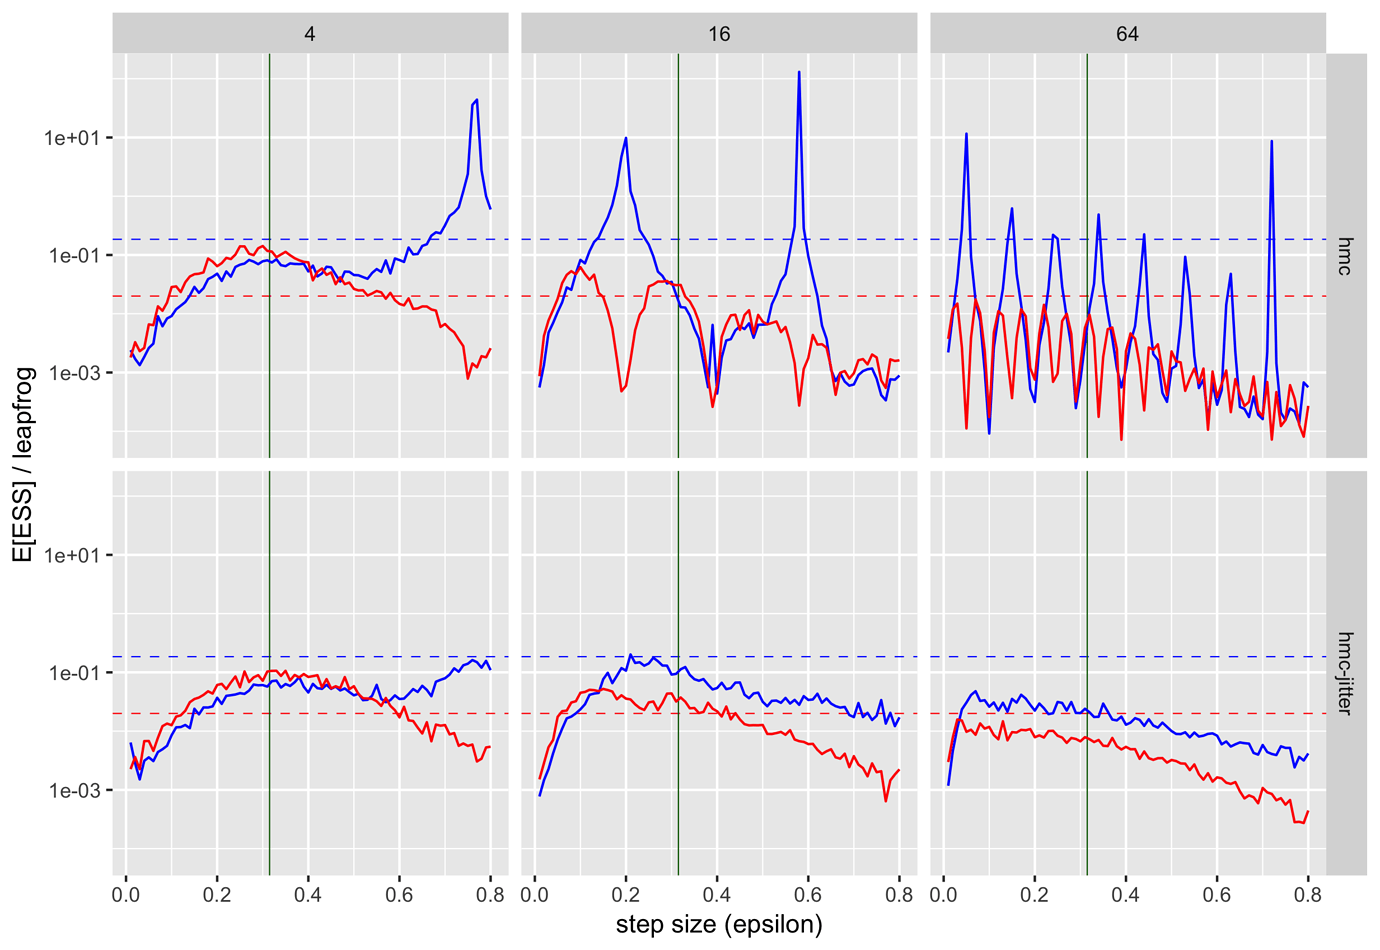
\includegraphics[width=\textwidth]{img/ess-per-leapfrog-jitter-hmc.png}
\end{minipage}%
\begin{minipage}[t]{0.29\textwidth}
  \null\vspace*{-2.5in}
  \begin{subitemize}
  \item \myemph{Target}: 1000-dim standard normal
  \item \myemph{y-axis} (log):  ESS; \\ \myemph{x-axis}: step size
  \item \myemph{blue}: $\mathbb{E}[\Theta]$; \\ \myemph{red}:
    $\mathbb{E}[\Theta^2]$
  \item \myemph{top}: HMC; \\ \myemph{bottom}: jittered time HMC
  \item \myemph{solid}:~HMC,\\ \myemph{dashed}: NUTS
  \end{subitemize}
\end{minipage}

\sld{Leapfrog integrator simulates trajectories}
\begin{itemize}
\item \myemph{Leapfrog step} from $(\theta(t), \rho(t))$ with step $\epsilon$, mass $M$
  \begin{eqnarray*}
    \rho(t + 1/2) & = & \rho(t) + \epsilon / 2 \cdot \nabla \log p(\theta(t))
    \\[4pt]
    \theta(t+1) & = & \theta(t) + \epsilon \cdot M^{-1} \cdot \rho(t + 1/2)
    \\[4pt]
    \rho(t + 1) & = & \rho(t + 1/2) + \epsilon / 2 \cdot \nabla \log p(\theta(t + 1)) 
  \end{eqnarray*}
\item \myemph{Stabile} if $\epsilon < 2 / \sqrt{\lambda^\text{max}}$, where $\lambda^\textrm{max}$ is max eigenvalue of Hessian,
  $$H(\theta) = \nabla \nabla^\top \! -\log p(\theta)$$
  \begin{subitemize}
  \item \myemph{local error}:  $\mathcal{O}(\epsilon^3)$
  \item \myemph{global error}: $\mathcal{O}(\epsilon^2)$
  \end{subitemize}
\end{itemize}

\sld{Multinomial HMC}
\begin{itemize}
\item \myemph{Each iteration} from previous position $\theta(0)$:
  \begin{subitemize}
  \item generate new momentum $\rho(0) \sim \textrm{normal}(0, M)$
  \item generate \myemph{random steps forward} $F \sim \textrm{uniform}(\{ 0, \ldots, L \})$
  \item take $B = L - F$ leapfrog \myemph{steps backward} and $F$ forward from
    $(\theta(0), \rho(0))$
  \item yields $(\theta(n), \rho(n))$ for $-B \leq n \leq F$
    (including initial)
  \item \myemph{randomly select next state} $(\theta(n), \rho(n))$ \\[4pt]
    with probability \myemph{proportional to density}, $\null \propto p(\theta(n), \rho(n))$
  \end{subitemize}
\item \myemph{No rejection}, \myemph{no harmonics}, and \myemph{no bad
    luck} due to error $\pm H(\theta(0), \rho(0))$
  \vfill
\item Straightforward to prove \myemph{detailed balance} (cf. our
  second \textit{GIST} paper)
\end{itemize}

\sld{Naive no-U-turn sampler (NUTS)}
\begin{itemize}
\item Go forward or backward uniformly at random,
\item doubling number of steps each time,
\item until there is a U-turn between ends (i.e., ends heading toward each other).
\item But, if there is a sub-U-turn in the new states, throw away new doubling.
  \begin{subitemize}
  \item inefficient, but necessary for detailed balance
  \end{subitemize}
\item select next state proportional to density (a la multinomial HMC)
  \vfill
\item Original naive NUTS: slice sample rather than multinomial sample
\end{itemize}

\sld{Biased-progressive NUTS}
\begin{itemize}
\item Keep a selected state, initially $z(0) = (\theta(0), \rho(0))$
\item At each doubling from $M$ to $2M$ states:
  \begin{subitemize}
    \item Extend $z(1), \ldots, z(M)$ to $z(1), \ldots, z(M), z(M+1), \ldots, z(2M)$
    \item Metropolis \myemph{probability of updating state}:
      $$
      1 \wedge
      \dfrac{p\!\left(z(M+1)\right) + \cdots + p\!\left(z(2M)\right)}
            {p\!\left(z(1)\right) + \cdots + p\!\left(z(M)\right)}
            $$
          \item If Hamiltonian simulation perfect, probability is 1.            
      \item If updating, \myemph{select new state} $z(m)$ 
        with probability \myemph{proportional to density},  $\propto p(z(m))$,
        from among candidate states $z(M+1), \ldots, z(2M)$.
  \end{subitemize}
\item Return final selected item.
\end{itemize}

\sld{Biased-progressive vs. naive jump distance}
\begin{center}
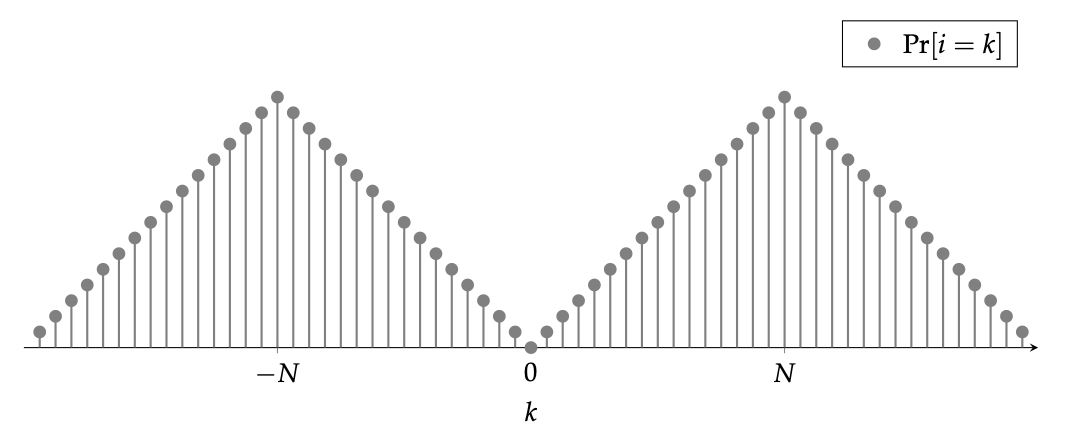
\includegraphics[width=0.6\textwidth]{img/multinomial-hmc-L.png}
\end{center}
\begin{itemize}
\item Assuming \myemph{perfect simulation} of the Hamiltonian trajectory, each state equally likely.
\item \myemph{Naive} NUTS and multinomial sample \myemph{uniformly} along trajectory.
\item \myemph{Biased-progressive} NUTS samples \myemph{as above} ($N = 2^M$ total steps)
\end{itemize}

\sld{Preconditioning with a mass matrix}
\begin{itemize}
\item The positive-definite \myemph{mass matrix} $M$ acts as a \myemph{global preconditioner}
\item If $\theta \sim \textrm{normal}(\mu, \Sigma)$, then $M = \Sigma^{-1}$ is a \myemph{perfect preconditioner}
  \begin{subitemize}
  \item i.e., mass-adjustment samples like standard normal
  \end{subitemize}
\item NUTS uses \myemph{fixed warmup iterations} with unit mass matrix before sampling to estimate $\textrm{cov}[\Theta]$
\item \myemph{Chicken-and-egg} problem:
  \begin{subitemize}
  \item need to sample efficiently to estimate mass matrix effectively
  \item need good mass matrix to sample efficiently
  \end{subitemize}
\item There are \myemph{better mass matrix estimators} than we used for Stan (see below).
\end{itemize}

\sld{The curse of varying geometry}
\begin{itemize}
\item If the Hessian varies, \myemph{global preconditioning fails}.
\item e.g., \myemph{Neal's funnel}: condition varies 0 to 1000+, eigenstructure varies 
\item By \myemph{adjusting step size} lower in neck (color), \myemph{WALNUTS succeeds}\\[12pt]
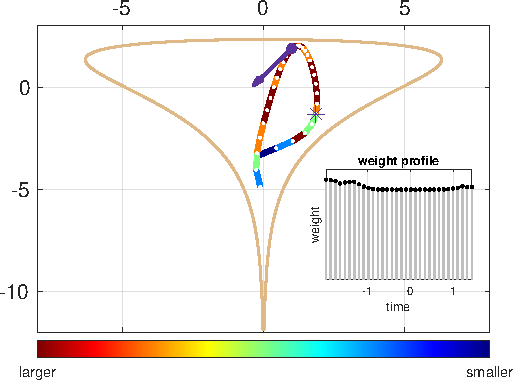
\includegraphics[width=0.32\textwidth]{img/funnel1.pdf}%
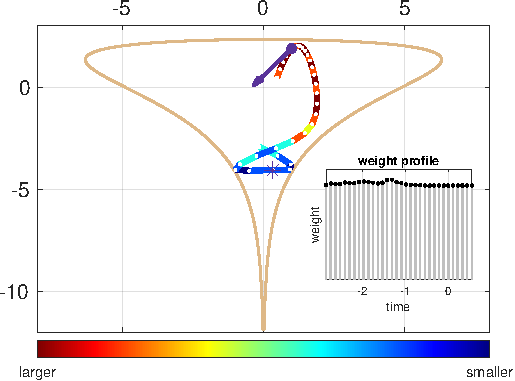
\includegraphics[width=0.32\textwidth]{img/funnel2.pdf}%
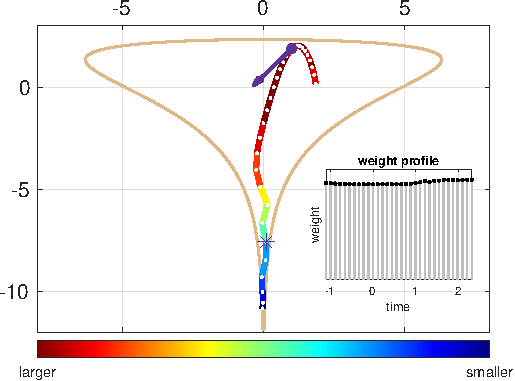
\includegraphics[width=0.32\textwidth]{img/funnel3.pdf}
\end{itemize}

\sld{Gibbs self tuning (GIST)}
\begin{itemize}
\item On the road to WALNUTS, we came up with \myemph{Gibbs self tuning} (Bou-Rabee, Marsden, me)
\item Add \myemph{auxiliary tuning} variables, e.g., $\alpha = L, \epsilon, M$ for HMC
\item \myemph{Gibbs sample} tuning parameters given state $\alpha \sim p(\alpha \mid \theta, rho)$
  \begin{subitemize}
  \item need to pick a reasonable conditional distribution
  \end{subitemize}
\item Use tuning parameters $\alpha$ with NUTS to \myemph{propose} $\theta(t), \rho(t)$
\item \myemph{Metropolis-within-Gibbs} accept:
  $$
  \Pr[\textrm{accept } \theta(t), \rho(t)]
  = \dfrac{p(\theta(t), \rho(t))}{\underbrace{p(\theta(0), \rho(0))}_\textrm{Metropolis}}
    \cdot 
    \dfrac{p(\alpha \mid \theta(t), \rho(t))}{\underbrace{p(\alpha \mid \theta(0), \rho(0))}_\textrm{correction}}
    $$
\end{itemize}

\sld{GIST II}
\begin{itemize}
\item We applied GIST to step size tuning (Bou-Rabee, Marsden, Kleppe, me)
\item Start at step size $\epsilon = \epsilon^\textrm{max}$
\item While selecting steps $L$ w.\ NUTS doesn't preserve Hamiltonian within $\tau$ between any two states on trajectory
  \begin{subitemize}
  \item $\epsilon = \epsilon / 2$
    \end{subitemize}
  \item \myemph{Correction is 1} if same number of halvings forward and backward; else reject.
    \vspace*{-12pt}
    \begin{subitemize}
    \item GIST technically allows further randomization around halvings.
    \end{subitemize}
  \vfill
  \item {\small Bou-Rabee, N., Carpenter, B., Kleppe, T.S. and Marsden, M., 2024. \myemph{Incorporating local step-size adaptivity into the No-U-Turn Sampler using Gibbs self tuning}. \textit{arXiv} 2408.08259.}
\end{itemize}

\sld{WALNUTS}
\begin{itemize}
\item Just like GIST II, but \myemph{every leapfrog step} \\[4pt]
  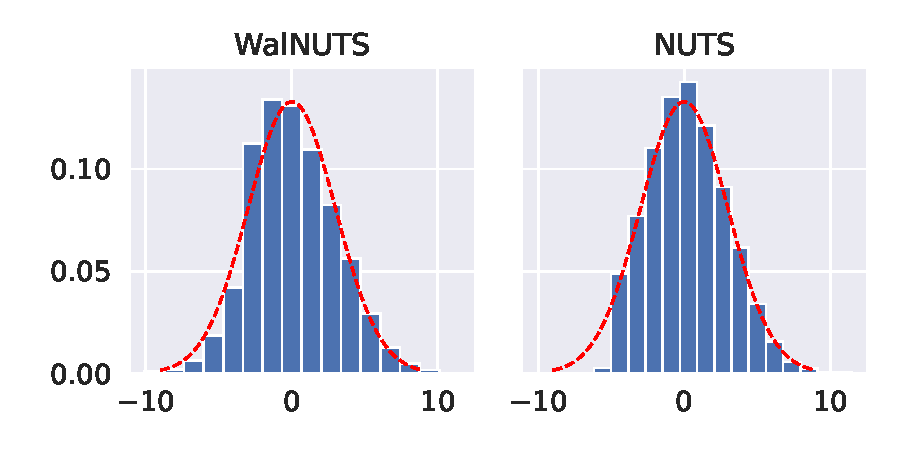
\includegraphics[width=0.55\textwidth]{img/funnel_hist.pdf}
  \vspace*{-4pt}
\item {\small \myemph{Et voila!}}
\item {\small Bou-Rabee, N., Carpenter, B., Kleppe, T.S. and Liu, S., 2025. \myemph{The Within-Orbit Adaptive Leapfrog No-U-Turn Sampler}. \textit{arXiv}:2506.18746.}
\end{itemize}

\sld{Adaptation in C++ code [WIP]}
\begin{itemize}
\item \myemph{Mass matrix}: A continuous, diagonal form of \myemph{Nutpie's mass matrix} adaptation scheme (Seyboldt et al.\ in prep)
  \begin{subitemize}
  \item Minimizes \myemph{Fisher divergence}, a form of \myemph{gradient divergence}
  \item uses \myemph{covariance of draws}, like NUTS,
  \item plus \myemph{covariance of scores}, which is inverse covariance in multi-normal
  \item \myemph{Initialize} at absolute gradient of log density (regularized outer product estimate)
  \end{subitemize}
\item \myemph{Max step size}: Use \myemph{dual averaging} a la NUTS for setting $\epsilon^\textrm{max}$ to target $2/3$ accept.
  \begin{subitemize}
    \item Any lower is suboptimal on computational grounds.
  \end{subitemize}
\end{itemize}

\sld{Next steps: local adaptation}
\begin{itemize}
\item \myemph{Local mass matrix} adaptation.
  \begin{subitemize}
  \item For \myemph{log concave} can use GIST with inverse Wishart distribution around negative Hessian of log density
  \item still expensive, even Cholesky factored.
  \item perhaps use \myemph{low rank plus diagonal} to reduce from $\mathcal{O}(N^3)$ to $\mathcal{O}(K^2 N)$.
  \item Nawaf Bou-Rabee has been exploring \myemph{explicit Riemannian} HMC schemes (stay tuned!).
    \end{subitemize}
\item \myemph{Local step size} adaptation.
\vfill
\begin{subitemize}
\item Perhaps follow Matt Hoffman and Pavel Sountsov's \myemph{CheeS HMC} to efficiently approximate \myemph{max eigenvalue}.
\end{subitemize}
\vfill
\item We're \myemph{open to suggestions}!
\end{itemize}

\sld{QR code for C++ source, paper, and slides}
\\[8pt]
\spc
\noindent
\begin{minipage}[t]{0.35\textwidth}

\includegraphics[width=\textwidth]{img/qr-code.pdf}
\end{minipage}
\quad
\begin{minipage}[t]{0.6\textwidth}
  \vspace*{-1.55in}
  {\small Nawawf Bou-Rabee, Bob Carpenter, Tore S. Kleppe, and Sifan Liu.
      2025. \myemph{WALNUTS: The Within-Orbit Adaptive Leapfrog No-U-Turn
      Sampler}. \textit{arXiv} 2506.18746.}
      \\[12pt]
      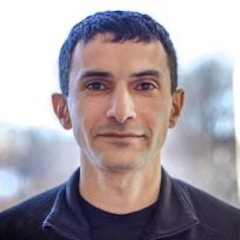
\includegraphics[width=0.25\textwidth]{img/nawaf.jpg}
      \hfill
      
\includegraphics[width=0.25\textwidth]{img/tore.png}
      \hfill
      
\includegraphics[width=0.25\textwidth]{img/sifan.jpg}
\end{minipage}
\hfill
\null



\end{document}